\section{编码对比}\label{sec:encodings}

本节在完全相同的物理条件下比较八种编码：同一个仿真器、同样的器件参数范围和光功率范围、同样的读出（31 根梳齿、8 个抽头）、
同样的噪声模型，以及同样数量的随机工作点和同样的选点流程（第~\ref{sec:protocol}~节）。
表~\ref{tab:encodings} 汇总了三个任务在无噪声和现实噪声下的结果，图~\ref{fig:encodings} 画出同样的数字。

% generated by experiments/make_table1.py; do not edit by hand
\begin{table}[htbp]
\centering
\caption{各编码与基线的测试误差（NMSE，越小越好）。每种编码在相同范围内各抽 256 个随机工作点，按新运行的平均验证误差选点，报告另外 6 组新运行的平均测试误差，再取 3 条序列的几何平均；读出层训练在一次运行上、测试在另一次噪声独立的运行上。每列最好的微环编码用粗体标出。ESN 与微环的读出维度相同（31 个节点、相同的延迟抽头），只用一个随机储备池，现实噪声下给它的输入噪声为 $3\times10^{-3}$；更强的软件基线见第~\ref{sec:software}~节。信道均衡在现实噪声下的测试段为 5000 个符号。}
\label{tab:encodings}
\small
\begin{tabular}{lcccccc}
\toprule
 & \multicolumn{2}{c}{Mackey--Glass（10 步预测）} & \multicolumn{2}{c}{非线性信道均衡} & \multicolumn{2}{c}{NARMA-10} \\
\cmidrule(lr){2-3}\cmidrule(lr){4-5}\cmidrule(lr){6-7}
编码 & 无噪声 & 现实噪声 & 无噪声 & 现实噪声 & 无噪声 & 现实噪声 \\
\midrule
泵浦功率~\cite{shishavan2025} & $0.20$ & $0.33$ & $7.6\times10^{-3}$ & $1.0\times10^{-2}$ & $0.21$ & $0.35$ \\
泵浦失谐~\cite{cuevas2025} & $5.6\times10^{-2}$ & $9.3\times10^{-2}$ & $1.2\times10^{-2}$ & $3.0\times10^{-2}$ & $0.21$ & $0.45$ \\
泵浦相位~\cite{arabieh2026soliton} & $0.14$ & $0.20$ & $4.8\times10^{-2}$ & $7.7\times10^{-2}$ & $0.66$ & $1.0$ \\
泵浦功率，孤子起点 & $1.9\times10^{-3}$ & $5.3\times10^{-2}$ & $1.1\times10^{-2}$ & $2.1\times10^{-2}$ & $0.20$ & $0.32$ \\
泵浦失谐，孤子起点 & $1.7\times10^{-3}$ & $9.5\times10^{-2}$ & $1.2\times10^{-2}$ & $0.17$ & $0.19$ & $0.39$ \\
泵浦相位，孤子起点 & $2.8\times10^{-3}$ & $5.0\times10^{-2}$ & $3.5\times10^{-2}$ & $6.0\times10^{-2}$ & $0.68$ & $0.74$ \\
整体调制光梳 & $8.2\times10^{-5}$ & $4.8\times10^{-3}$ & $5.0\times10^{-3}$ & $7.6\times10^{-3}$ & $0.18$ & $0.21$ \\
谱相位掩模（本文） & $\mathbf{1.8\times10^{-6}}$ & $\mathbf{3.3\times10^{-4}}$ & $\mathbf{3.7\times10^{-3}}$ & $\mathbf{5.7\times10^{-3}}$ & $\mathbf{0.16}$ & $\mathbf{0.19}$ \\
\midrule
ESN（31 节点） & $2.4\times10^{-5}$ & $3.2\times10^{-4}$ & $3.8\times10^{-3}$ & $4.0\times10^{-3}$ & $0.11$ & $0.11$ \\
线性自回归 & $0.14$ & $0.21$ & $1.1\times10^{-2}$ & $1.3\times10^{-2}$ & $0.19$ & $0.19$ \\
\bottomrule
\end{tabular}
\end{table}


\begin{figure}[htbp]
\centering
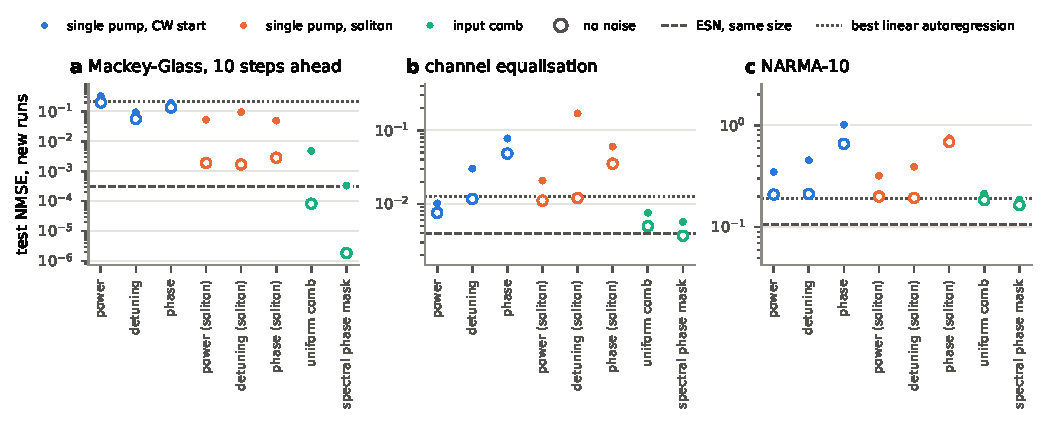
\includegraphics[width=\linewidth]{fig4_encodings}
\caption{现实噪声下八种编码在三个任务上的测试误差（表~\ref{tab:encodings} 的“现实噪声”列；新运行复测，3 条序列的几何平均）。
蓝色：从零场起振的单泵浦编码；橙色：从单孤子出发的单泵浦编码；绿色：输入光梳（整体调制和谱相位掩模）。
虚线为同读出维度的 ESN（输入噪声 $3\times10^{-3}$），点线为最好的线性自回归。
（a）Mackey--Glass 10 步预测；（b）非线性信道均衡；（c）NARMA-10。}
\label{fig:encodings}
\end{figure}

\subsection{Mackey--Glass 预测}

谱相位掩模在 Mackey--Glass 上的优势最大。无噪声时它的测试误差为 $1.8\times10^{-6}$，
比整体调制的光梳（$8.2\times10^{-5}$）好约 45 倍，比最好的单泵浦编码（从孤子出发的失谐编码，$1.7\times10^{-3}$）好约 900 倍，
比从零场起振的单泵浦编码好四到五个数量级。
现实噪声下所有编码都变差，但次序不变：掩模为 $3.3\times10^{-4}$，整体调制的光梳为 $4.8\times10^{-3}$（差约 15 倍），
最好的单泵浦编码为 $5.0\times10^{-2}$（差约 150 倍）。

同读出维度的 ESN 在无噪声时为 $2.4\times10^{-5}$，掩模比它好约 13 倍；
现实噪声下 ESN 为 $3.2\times10^{-4}$，与掩模持平。
后一个比较依赖于给 ESN 设定的输入噪声：这里用的是 $3\times10^{-3}$，而且 ESN 只用了一个随机储备池；
多试几个储备池后 ESN 降到 $1.9\times10^{-4}$，输入噪声降到 $10^{-3}$ 时更降到 $5.3\times10^{-5}$。
第~\ref{sec:software}~节专门讨论这种比较，本节只比较光学编码之间的差别，它们共享同一套噪声模型，不受这个约定影响。

\subsection{优势不是来自单个幸运的工作点}

一种编码的最好结果，可能只是在 256 次随机抽取中碰上了一个特别好的点。
图~\ref{fig:distributions} 给出每种编码全部随机工作点的误差分布（现实噪声下的 Mackey--Glass，3 条序列共 768 个点）。
掩模的整个分布都明显左移：它的中位数为 $4.3\times10^{-2}$，已经好于每一种单泵浦编码最好的那 10\% 的点（$0.14$ 到 $0.38$）；
最好的 10\% 掩模工作点低于 $1.9\times10^{-3}$，比整体调制光梳最好的 10\%（$2.5\times10^{-2}$）好一个数量级以上。
所以掩模的优势是这一类输入方式整体的性质，不依赖于某个特别的参数组合。

\begin{figure}[htbp]
\centering
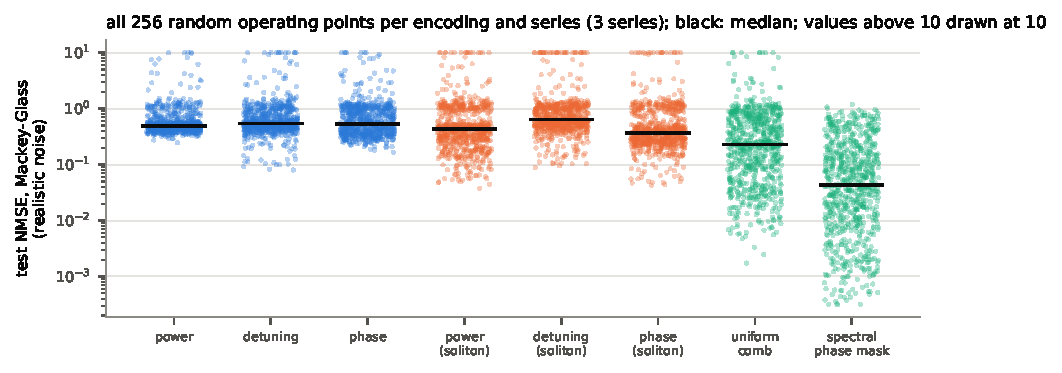
\includegraphics[width=\linewidth]{fig5_distributions}
\caption{现实噪声下 Mackey--Glass 的测试误差分布：每种编码每条序列 256 个随机工作点（3 条序列共 768 个点，每点一对运行），黑线为中位数；
高于 10 的值画在 10 处。颜色与图~\ref{fig:encodings} 相同。}
\label{fig:distributions}
\end{figure}

\subsection{信道均衡}

信道均衡上的差别小得多。掩模仍是最好的光学编码，无噪声时为 $3.7\times10^{-3}$，现实噪声下为 $5.7\times10^{-3}$，
比整体调制的光梳好约 1.3 倍，比最好的单泵浦编码（功率编码）好约 2 倍，比线性自回归（$1.1\times10^{-2}$ 和 $1.3\times10^{-2}$）好 2 到 3 倍。
无噪声时掩模与 ESN（$3.8\times10^{-3}$）持平；现实噪声下 ESN 为 $4.0\times10^{-3}$，比掩模好约 1.4 倍。
这个任务的误差主要来自信道本身的噪声，第~\ref{sec:software}~节显示，把 ESN 的输入噪声降到零它也只改善约 7\%。
按误符号率看（每条序列 6 组新运行、每组 5000 个测试符号，3 条序列共 9 万个符号），掩模为 $1.9\times10^{-4}$（17 个错误），
整体调制的光梳为 $1.0\times10^{-4}$（9 个），功率编码为 $3.9\times10^{-4}$（35 个），ESN 为 $1.1\times10^{-5}$（1 个）。
掩模与整体调制的光梳在这个统计量下分不开；所有光梳编码和 ESN 都远低于常用的硬判决纠错门限 $3.8\times10^{-3}$。

\subsection{NARMA-10：单环不成立的例子}

NARMA-10 需要约 10 个符号的记忆，而微环自身的记忆只有光子寿命，几个符号以内。
单个微环上，掩模（无噪声 $0.16$，现实噪声 $0.19$）只与线性自回归（$0.19$）持平，略好于整体调制的光梳和单泵浦编码，
但比 ESN（$0.11$）差约 1.5 到 1.8 倍。我们把它作为不成立的例子如实报告。
记忆可以从外部补上：给输入梳齿再加一份延迟后的信号（输入延迟线），并把几个掩模不同的环拼接读出后，
NARMA-10 降到 $0.011$，与带同样延迟线的 100 节点 ESN（$0.010$）持平（第~\ref{sec:memory}~节和补充材料）。

\subsection{起作用的是梳齿相位的随机性}\label{sec:ablation}

为了弄清掩模的哪一部分在起作用，我们在相同的工作点范围内比较了几种简化的掩模（现实噪声，与表~\ref{tab:encodings} 相同的流程；补充图 S1）。
在 Mackey--Glass 上：
\begin{itemize}
\item 只让相位随机、所有梳齿幅度相同的掩模为 $2.4\times10^{-4}$，与完整掩模（这组运行中为 $3.8\times10^{-4}$）一样好或略好；
\item 只让幅度随机、所有梳齿同相的掩模为 $1.3\times10^{-3}$，差 3 到 6 倍；
\item 随机的静态光谱加一个统一的调制（$w_\mu\propto b_\mu$）为 $6.5\times10^{-4}$；
\item 幅度和相位都相同的整体调制为 $5.0\times10^{-3}$。
\end{itemize}
信道均衡上的次序相同（只调相位 $5.0\times10^{-3}$，完整掩模 $5.4\times10^{-3}$，只调幅度 $5.8\times10^{-3}$，整体调制 $7.3\times10^{-3}$），只是差别更小。
输入梳齿的数量也有影响：Mackey--Glass 上 4、8、16、32、64 根分别为
$1.9\times10^{-3}$、$1.4\times10^{-3}$、$3.8\times10^{-4}$、$2.4\times10^{-4}$、$2.1\times10^{-4}$，32 根以后不再明显改善；
信道均衡上 32 根最好（$4.0\times10^{-3}$），64 根反而变差（$5.6\times10^{-3}$）。

这给出第一条设计规则：\emph{起作用的是各梳齿相位的随机性，而不是每根梳齿独立的幅度调制}。
实现上不需要逐梳齿的调制器，一个调制器加两个只设相位的谱整形器就够了。
为什么相位比幅度重要，我们还没有完整的解释。一个直观的猜想是：随机相位让不同梳齿经四波混频进入同一根输出梳齿的各条路径以不同方式干涉，
使各输出梳齿的特征彼此更不相关。但这个猜想在线性层面上不成立。我们在每种变体选出的工作点上（无噪声，Mackey--Glass）计算了 31 路特征的相关矩阵：
有效秩（参与率，特征值之和的平方除以特征值平方之和）在整体调制、随机谱加统一调制、只调幅度、只调相位和完整掩模之间分别为
$2.2$、$2.3$、$2.4$、$2.2$、$2.0$，平均相关系数的绝对值为 $0.58$、$0.58$、$0.57$、$0.60$、$0.65$，几种变体几乎相同，完整掩模的线性多样性甚至最低。
所以掩模的好处不在于瞬时特征之间的线性去相关，而更可能在于各特征是输入历史的不同的高阶非线性函数；这需要用信息处理容量一类的分解来检验，留作后续工作。
